% ai-phishing-detection-dissertation/report/sections/4-results/distilbert-model-performance/performance-on-internal-test-set.tex

\subsubsection*{Performance on internal test set}
The DistilBERT model, via "\texttt{distilbert-base-uncased}", was fine-tuned on 29,280 samples of the training portion, i.e. the combined Enron (ham) and CEAS 2008 (spam), for 3 epochs. The entire training process took approximately \textbf{34 minutes} on a Tesla T4 GPU. For each epoch:

\begin{itemize}
  \item \textbf{Epoch 1}:
  \begin{itemize}
    \item \textit{Average training loss}: 0.0505
    \item \textit{Validation loss}: 0.0166
    \item \textit{Validation accuracy}: 0.9959
    \item \textit{Validation F1-score}: 0.9959
    \item \textit{Duration}: approx. 633 seconds
  \end{itemize}
  \item \textbf{Epoch 2}:
  \begin{itemize}
    \item \textit{Average training loss}: 0.0091
    \item \textit{Validation loss}: 0.0159
    \item \textit{Validation accuracy}: 0.9965
    \item \textit{Validation F1-score}: 0.9965
    \item \textit{Duration}: approx. 637 seconds
  \end{itemize}
  \item \textbf{Epoch 3}:
  \begin{itemize}
    \item \textit{Average training loss}: 0.0023
    \item \textit{Validation loss}: 0.0139
    \item \textit{Validation accuracy}: 0.9974
    \item \textit{Validation F1-score}: 0.9974
    \item \textit{Duration}: approx. 637 seconds
  \end{itemize}
\end{itemize}

\noindent The best performing epoch is selected, that being \textbf{Epoch 3}, for the DistilBERT model to be fine-tuned upon the internal test set comprising of 6,275 samples. The performance metrics on the internal test set are as follows:

\begin{table}[h]
\centering
\begin{tabularx}{\textwidth}{|X|X|}
\hline
\textbf{Metric} & \textbf{Value} \\
\hline
Accuracy & \texttt{0.9973} \\
\hline
Precision (Phishing) & \texttt{0.9979} \\
\hline
Recall (Phishing) & \texttt{0.9969} \\
\hline
F1-Score (Phishing) & \texttt{0.9974} \\
\hline
ROC AUC Score  & \texttt{1.0000} \\
\hline
\end{tabularx}
\caption{Random Forest performance on combined dataset}
\end{table}

\noindent The confusion matrix is presented below.

\begin{figure}[H]
  \begin{center}
    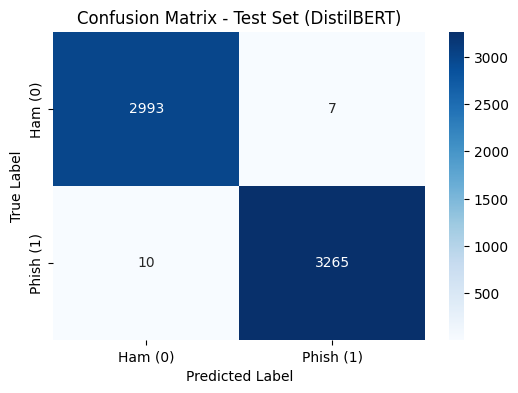
\includegraphics[scale=0.85]{confusion-matrices/distilbert/internal-test-set.png}
    \caption{Confusion matrix for DistilBERT internal test set}
  \end{center}
\end{figure}

\noindent The classification report presented below provides further insights.

\begin{table}[h]
\centering
\begin{tabularx}{\textwidth}{|X|X|X|X|X|}
\hline
\textbf{Class} & \textbf{Precision} & \textbf{Recall} & \textbf{F1-Score} & \textbf{Support} \\
\hline
Ham (0) & \texttt{1.00} & \texttt{1.00} & \texttt{1.00} & \texttt{3000} \\
\hline
Phish (1) & \texttt{1.00} & \texttt{1.00} & \texttt{1.00} & \texttt{3275} \\
\hline
Accuracy & & & \texttt{1.00} & \texttt{6275} \\
\hline
Macro Avg & \texttt{1.00} & \texttt{1.00} & \texttt{1.00} & \texttt{6275} \\
\hline
Weighted Avg & \texttt{1.00} & \texttt{1.00} & \texttt{1.00} & \texttt{6275} \\
\hline
\end{tabularx}
\caption{DistilBERT classification report on internal test set}
\end{table}

\noindent From these results, it can be said that DistilBERT demonstrated exceptionally high performance on the internal test set, due to its near perfect scores across all metrics.
